%! Author = dayan3847
%! Date = 5/13/23

% Preamble
\documentclass[11pt]{article}

% Packages
\usepackage{amsmath}
\usepackage{graphicx}

% Document
\begin{document}

    Universidad Autónoma de Yucatán

    Dayan Bravo Fraga

    Machine Learning

    Teacher: Dr. Victor Uc Cetina

    Student: Dayan Bravo Fraga


    \section{Task1: Stochastic Gradient Descent}\enumer

    GitHub: https://github.com/dayan3847/machine_learning/tree/master/stochastic_gradient_descent

    Final Report

    Final model with optimal learned parameters.

    Polynomial Degree: 10

    h(x) =+0.13446691950596312 * X^0+5.639362010213212 * X^1-9.683392522200206 * X^2-4.612341933382566 * X^3+0.631841522059667 * X^4+3.3153792664891295 * X^5+3.9201858682240904 * X^6+2.297355998185093 * X^7+1.263616418845794 * X^8-0.9212010227127019 * X^9-1.621848037352991 * X^10Alpha = 0.1

    Graphs

    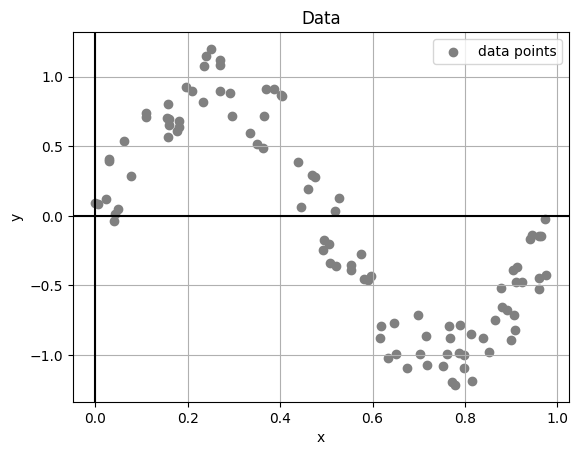
\includegraphics[width=0.5\textwidth]{../img/output1.png}

    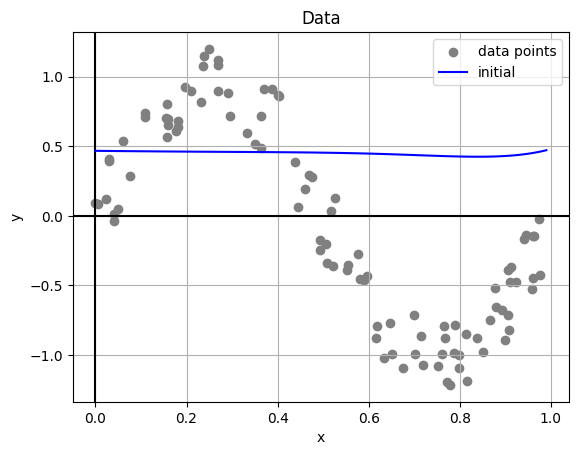
\includegraphics[width=0.5\textwidth]{../img/output2.png}

    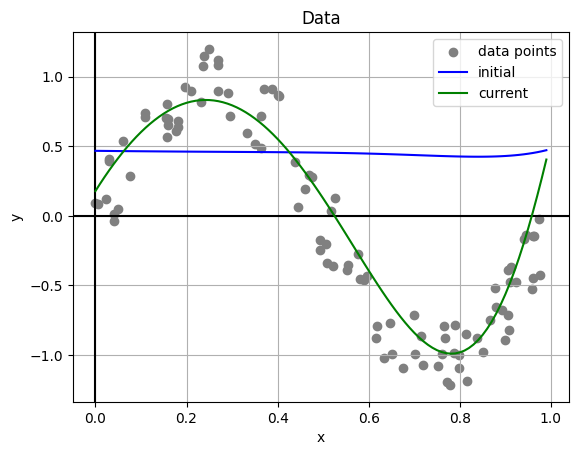
\includegraphics[width=0.5\textwidth]{../img/output3.png}

    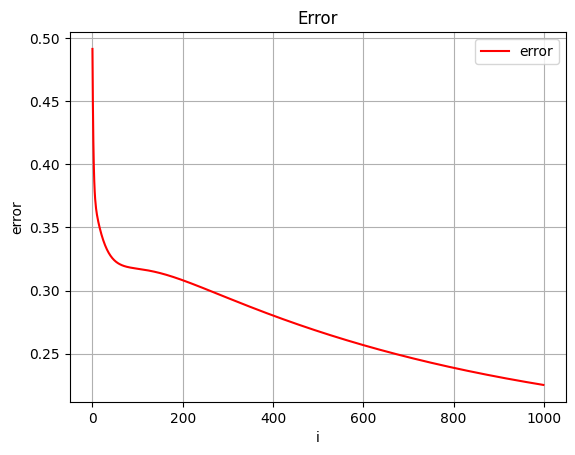
\includegraphics[width=0.5\textwidth]{../img/output4.png}

\end{document}